\subsection{Eksperimenta protokols: FAST CPU implementāciju salīdzinājums}\label{appx:test1}
\setcounter{table}{0} %Reset table counter for (sub)appendix
\setcounter{figure}{0} %Reset figure counter for (sub)appendix
Eksperimenta mērķis ir salīdzināt
eksistējošo FAST algoritma implementāciju ātrdarbību CPU platformai, 
dodot iespēju izvērtēt implementācijas detaļas vadoties 
pēc kvantitatīva rādītāja. Iegūtie rezultāti arī uzstāda ātrdarbības 
,,etalonu'' GPU un FPGA platformu implementācijām.

Eksperiments tika veikts uz vairākiem datoriem, kuru aprīkojums norādīts
\ref{tbl:test1-dev}~tabulā. Izmantotie datori nosedz vairākas procesoru
sēriju paaudzes, kā arī reprezentē dažādas veiktspējas ,,spektra'' daļas.
\begin{table}[hb]\footnotesize
	\centering
	\caption{Izmantotās iekārtas (datori).}
	\label{tbl:test1-dev}
	\vspace{4pt}
	\begin{tabular}{cllll}
		\toprule
		\textbf{Nr.} & \textbf{Procesors} & \textbf{Takts frekvence} & 
			\textbf{Operētājsistēma} & \textbf{Arhitektūra}\\
		\midrule
		I & AMD Phenom 9950 & 2.60 GHz & Linux 3.10.7 (Gentoo) & \texttt{x86\_64}\\
		II & Intel Pentium M 740 & 1.73 GHz & Linux 3.10.17 (Gentoo) & \texttt{x86}\\
		III & Intel Core i5-2430M & 2.40 GHz & Windows 7 (+cygwin) & \texttt{x86\_64}\\
		IV & AMD Phenom II X6 1150T & 2.80 GHz & Linux 3.8.0 (Ubuntu) & \texttt{x84\_64}\\
		\bottomrule
	\end{tabular}
\end{table}

\begin{table}[hb]\footnotesize
	\centering
	\caption{Ātrdarbības rezultāti.}
	\label{tbl:test1-data}
	\vspace{4pt}
	\begin{tabular}{clcccrr}
		\toprule
		\input{results1-t1.tbl_tex}
		\bottomrule
	\end{tabular}
\end{table}
\footnotetext[1]{Kadri sekundē (angļu \termEn{frames per second}).}
\footnotetext{Miljoni pikseļu sekundē.}

Par ieejas datiem tika izmantota ,,\termEn{bas-relief}'' attēlu kopa%
	\footnote{Pieejama no \url{http://www.edwardrosten.com/work/junk.tar}},
kuru Rostens~un~Dramonds\cite{FAST} izmantoja FAST atkārtojamības testiem.
Uzstādītais jutības slieksnis $t$ visos testos bija 25, un katra 
attēla, iekārtas un implementācijas testa permutācija tika atkārtota 10 reizes.
Lielā datu apjoma dēļ (600 ieraksti) visa kopa netiek atspoguļota. Datu
apkopojums redzams \ref{tbl:test1-data}~tabulā, kur ,,Vid.~max'' kolonna
atspoguļo augstāko vērtību no kopas attēlu vidējiem rādītājiem
(t.i., ,,grūtākā'' kopas attēla vidējais apstrādes laiks 10 mērījumos).
,,Min'' un ,,Max'' kolonnas atspoguļo attiecīgi absolūto minimumu un absolūto
maksimumu no (80) uzņemto mērījumu sērijas.

\begin{figure}[tbh]
	\centering
	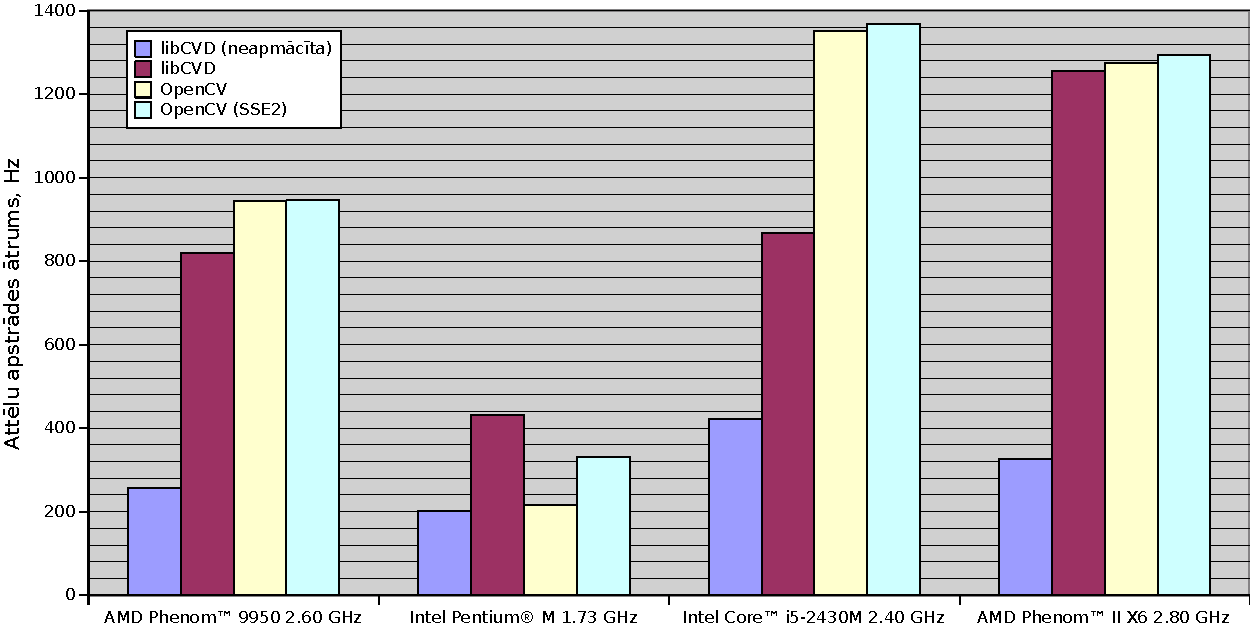
\includegraphics[width=\linewidth]{chart-cpu}
	\caption{Ātrdarbība dažādām implementācijām dažādās ierīcēs.}
	\label{fig:test1-data}
\end{figure}

Apskatot rezultātus (\ref{tbl:test1-data}~tabulu vai \ref{fig:test1-data}~attēlu)
ir veicami vairāki interesanti novērojumi. Lai gan CVD un OpenCV implementāciju
ātrdarbības uzlabojums pār neapmācīto CVD versiju bija paredzēts, to
savstarpējās atšķirības ir neparedzēti nekonsistentas.

Pirmkārt, CVD bibliotēkas implementācijas ātrdarbība ir augstāka uz vecas
paaudzes Pentium, bet jaunāko paaudžu procesoriem to pārspēj OpenCV
implementācija. Tas skaidrojams ar jaunāko paaudžu procesoru
SSE2 instrukciju kopas izpildes ātruma uzlabojumiem.

Otrkārt, OpenCV SSE2 versija sniedz tikai minimālus uzlabojumus ierīcēm
I, III un IV. Pēc papildus analīzes konstatēts, ka GCC kompilators,
pēc noklusējuma, 64~bitu sistēmām, iespējo SSE un SSE2 optimizāciju,
neatkarīgi no to atspējošanas ,,CMake'' vidē.
Tādējādi ,,neoptimizētā OpenCV'' rezultāti
šīm ierīcēm nav uzskatāmi par korektiem, un SSE2 uzlabojuma
salīdzināšanai nepieciešams testu atkārtot ar atspējotu SSE2 optimizāciju
kompilatora līmenī.
